\section{Definitions and nomenclature}
\label{sec:definitions}
\subsection{Systems and Stability}
In order to define stable learning algorithms, it is imperative to first recall the definition of first-order systems and stability, which is taken from \cite{khalil_nonlinear_2002}.

\begin{definition}[First-Order System]
 A continuous-time first-order system is defined by the following map
    \begin{equation}
    f:\mathbb{R}\times\mathbb{R}\rightarrow \mathbb{R}, (x(t),u(t)) \mapsto \dot x(t) = f(x(t),u(t)).
    \label{def:eq-system}
    \end{equation}

 Additionally, if $u(t)$ is a function of $x$, the system is autonomous, with closed-loop dynamics $f(x(t)$). The trajectory of the system is defined by the evolution of $x(t)$. Furthermore, the system has an equilibrium point at $f(x(t))=0$.
    \label{def:system}
\end{definition}

\begin{definition}[Stability]
 Consider the equilibrium point $x=0$ of \eqref{def:eq-system}. Then the system is:
 \begin{itemize}
 \item \textit{stable}, if for every $\epsilon>0$, there is a $\delta>0$, such that
     $$||x(0)||<\delta \Rightarrow ||x(t)||<\epsilon, \quad \forall t \geq 0$$ 
 \item \textit{unstable}, if not stable, and
 \item \textit{asymptotically stable} if it is stable and $\delta$ can be chosen such that
     $$||x(0)||<\delta \Rightarrow \lim_{t\rightarrow\infty} x(t)=0 $$
 \end{itemize} 
\end{definition}
Henceforth, the dependency of the dynamics on time is considered to be implicit and will be neglected in the notation.


\begin{definition}[Lyapunov function]
 A Lyapunov function is a continuous function $V: \mathbb{R}^n\rightarrow\mathbb{R}$ with the following properties:
 \begin{enumerate}
  \item[(a)] positive definitness: $V(x)>0, \quad \forall x\in\mathbb{R}^n\setminus\{0\}$ and $V(0)=0$,
  \item[(b)] decrease condition: $\dot V(x)\leq0, \quad \forall x\in\mathbb{R}^n$.
 \end{enumerate}
\end{definition}

\begin{definition}[Stability in the sense of Lyapunov]
 If there exists a continuous function $V: \mathbb{R}^n \rightarrow \mathbb{R}$ such that
    \begin{enumerate}
     \item[(a)] $V(x)$ is positive definite, and
     \item[(b)] $\dot{V}(x)\leq-l(x)$, for some positive semidefinite function $l(x)$,
    \end{enumerate}
 then the system is considered to be stable. Additionally, if $l(x)$ is positive definite, then the system is asymptotically stable.
    \label{def:lyapunov-stability}
\end{definition}

The ultimate goal of this work is to develop stable update laws for NNCs. Hence, the designed control law will be considered as a NN. Therefore, the following definition of NNs is used throughout this work.

\begin{definition}[Neural network]
 A neural network (NN) $\phi:\mathbb{R}^n\rightarrow \mathbb{R}^p$ is defined as:
\begin{equation}
 \begin{aligned}
 \phi (x) & = (L_{H} \circ \varphi_{H} \dots \circ L_{2} \circ \varphi_{2} \circ L_{1} \circ \varphi_1)(x)\\
 L_i(x) &= \theta_i x + b_i \quad \forall i\in\{1,..., H\},
\end{aligned}
\end{equation}
 where the activation functions are called $\varphi_i(\cdot)$, $\theta_i$ and $b_i$ are the weight matrix and bias of layer $i$, respectively. Whenever a bias is not mentioned it is assumed to be zero.
\end{definition}

NNs usually make use of nonlinear activation functions, which enable them to approximate nonlinear functions. Typically, functions such as the hyperbolic tangent, sigmoid, or ReLU are used in machine learning. This work will utilize an activation function that is designed to model a smooth saturation function, as used in \cite{wahby_enhanced_2024, thanhNonlinearPIDControl2006} and defined in \eqref{eq:sigmoid}. Note that the activation function saturates at $\pm \frac{2}{a}$.

\begin{equation}
 \sigma (x) = \frac{2(1-e^{-ax})}{a(1+e^{-ax})}
 \label{eq:sigmoid}
\end{equation}


\section{Nonlinear Model Reference Adaptive Control (NMRAC)}
\label{sec:NMRAC}
Direct MRAC is characterized by the controller parameters being directly updated through a mechanism, which takes into account the error of the system with respect to the desired output, as shown in Fig. \ref{fig:nonlinear-NNC-MRAC}. Furthermore, stability can be guaranteed through imposing that the conditions of Definition \ref{def:lyapunov-stability} are satisfied. In this section, the update law for NMRAC for first-order systems is derived.

\begin{figure}[!t]
 \centering
 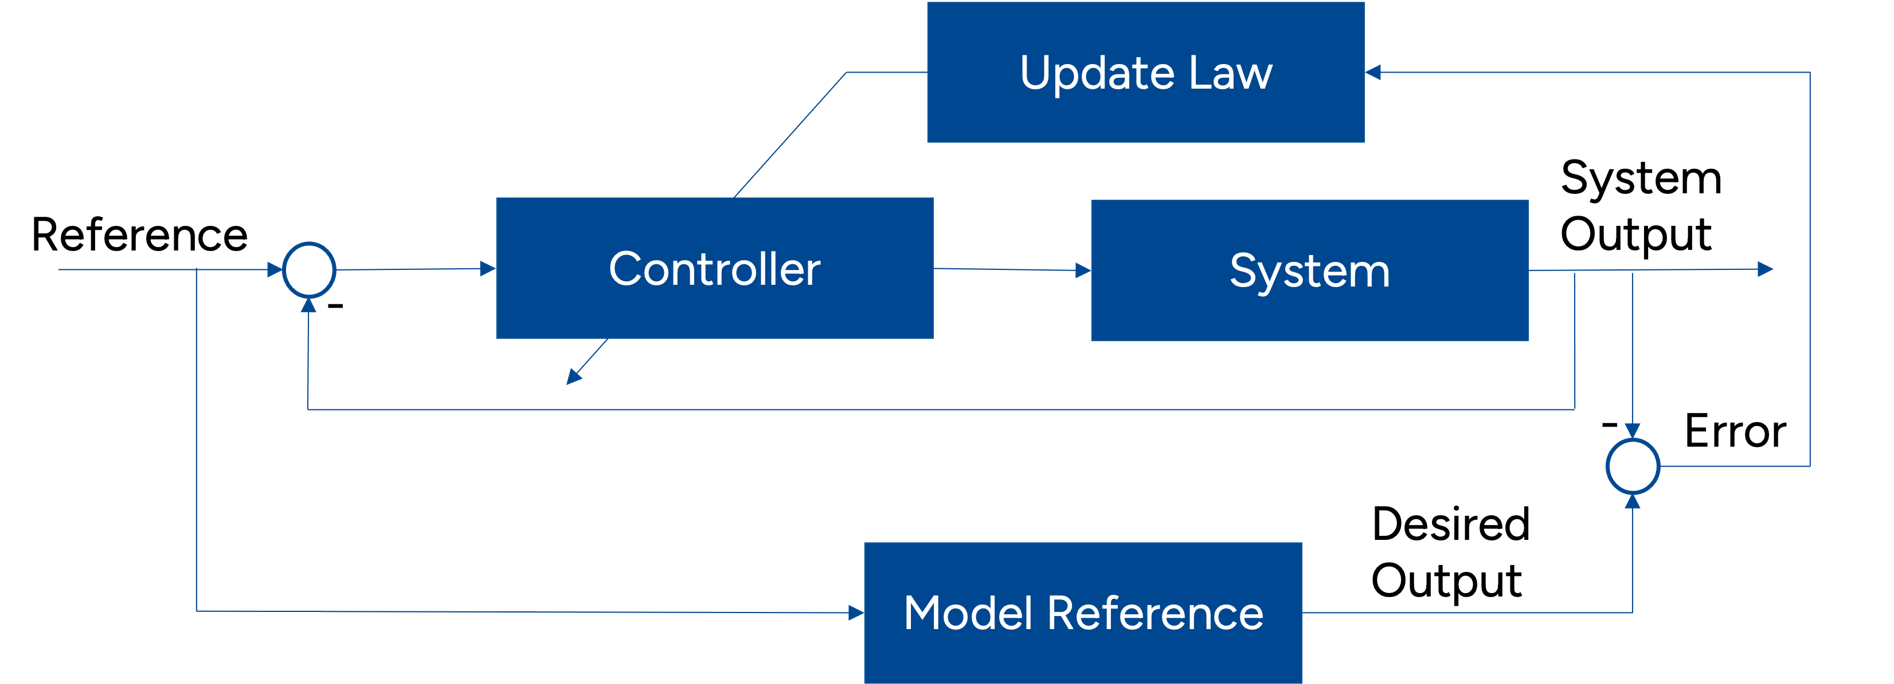
\includegraphics[width=0.8\linewidth]{images/MRAC_Blockdiagram.png}
 \caption{General direct MRAC schematic}
 \label{fig:nonlinear-NNC-MRAC}
\end{figure}

% In this work a stable update scheme is proposed for first-order systems. More, specifically, a problem is defined, where we show that even in the nonlinear case, we are able to learn a parameter with an algorithm that is based on the logic of a linear MRAC. We call this nonlinear Model Reference Adaptive Control (NMRAC).

The first-order system to control, as defined in Defintion \ref{def:system}, is parameterized as follows:
\begin{equation}
 \dot x = -ax + b\sigma(\theta e_x)
 \label{eq:first-order-system}
\end{equation}
where the NN $\phi: \mathbb{R}\rightarrow\mathbb{R}, \phi(x)=\sigma(\theta e_x)$ defines the control input, with an adaptable parameter $\theta$ and the state-tracking error $e_x=x_r - x$. Note that the activation function $\varphi$ is defined to be a smooth saturation function, as in \eqref{eq:sigmoid}. 

Next, a stable model reference is defined, as follows:
\begin{equation}
 \dot x_m = -a_mx_m + b_m\sigma_m(\theta_m e_m)
 \label{eq:first-order-ref}
\end{equation}
where $e_m=x_r - x_m$, and $a_m>0$.

Since the goal is that the system learns the behavior of the model reference, error dynamics is defined as follows:
\begin{equation}
 e=x_m-x
 \label{eq:error-dynamics-nonlinear}
\end{equation}
Note that from this definition it follows that $e=e_x-e_m$, which is used as an alternative definition for the stability analysis of the update law later on in this work.

Following the error dynamics, a Lyapunov candidate is defined as follows:
\begin{equation}
 V(e, \alpha) =||e||_2^2 + ||c \alpha||_2^2
 \label{eq:nonlinear-lyapunov-candidate}
\end{equation}
The factor $c>0$ can be considered to be the learning rate, which is used to accelerate or decelerate the learning process. The norm of the error $||e||_2^2$ captures the distance between the internal states of the model reference and the system, and the term $||\alpha||_2^2$ captures the distance between the NNC and the desired NNC, which can be seen as the difference in dynamics between the controlled system and the model reference. Note that both $e$ and $\alpha$ should be $0$ when the system follows the model reference and when the desired parameters are learned. This property renders our Lyapunov candidate in \eqref{eq:nonlinear-lyapunov-candidate} to be positive definite.

To ensure that the controlled system is stable, a negative time derivative of the Lyapunov function is required. Therefore, we analyze the behavior of the resulting time derivative of the Lyapunov function. The resulting equation is defined by \eqref{eq:nonlinear-lyapunov-derivative}.
\begin{equation}
 \begin{aligned}
 \dot V(e, \alpha) = & 2e\dot e + 2\alpha \dot \alpha c
 \end{aligned}
 \label{eq:nonlinear-lyapunov-derivative}
\end{equation}

The time derivative of the error dynamics is defined by \eqref{eq:nonlinear-error-time-derivative}. The equation is extended by $\pm (a_mx b_m \sigma_m(\theta_m e_x))$, to construct the term $\alpha$, which is now dependent on $e_x$, and $\theta$. Two terms remain, namely, $-a_me$, and $\gamma_m(e_m, e_x)$.

\begin{equation}
    \begin{aligned}
    \dot e 
= & \dot x_m - \dot x \\ 
= & -a_mx_m + b_m\sigma_m(\theta_me_m) - (-ax + b\sigma(\theta e_x)) \\
    & \pm (a_mx + b_m \sigma_m(\theta_m e_x)) \\
    = & -a_m \underbrace{(x_m-x)}_{=e} \\ 
    & + \underbrace{(a-a_m)x+b_m\sigma_m(\theta_me_x) - b\sigma(\theta e_x)}_{=\alpha(e_x, \theta)} \\ 
    & + \underbrace{b_m(\sigma_m(\theta_m e_m)-\sigma_m(\theta_m e_x))}_{=\gamma_m(e_m,e_x)}
    \end{aligned}
    \label{eq:nonlinear-error-time-derivative}
\end{equation}

Through substitution of \eqref{eq:nonlinear-error-time-derivative} into \eqref{eq:nonlinear-lyapunov-derivative}, equation \eqref{eq:nonlinear-lyapunov-derivative2} is obtained.
\begin{equation}
    \begin{aligned}
    \dot V(e, \alpha) 
    = & 2e(-a_me + \alpha(e_x, \theta) + \gamma_m(e_m, e_x)) + 2\alpha c \dot \alpha(e_x, \theta)\\
    = & -2a_me^2 \\ 
    & + 2e\gamma_m(e_m, e_x) 
    \\ 
    & + 2\alpha(e_x, \theta)(e + c \dot \alpha(e_x, \theta))
    \end{aligned}
    \label{eq:nonlinear-lyapunov-derivative2}
\end{equation}
Note that the first term $-2a_me^2$ is always negative, since $a_m>0$, and $e^2 > 0$. The second term will always be negative, due to the property of $e=e_x-e_m$. It follows that if $e<0 \Rightarrow \gamma_m(e_m, e_x)>0$, which implies that the second term is negative, and if $e>0 \Rightarrow \gamma_m(e_m, e_x)<0$, which again implies that the second term is negative. Hence, the second term always stays negative.

It remains to show that the last term does not influence equation \eqref{eq:nonlinear-lyapunov-derivative2} such that it changes sign. Since $\theta$ is dependent on time, this implies $\dot \alpha(e_x, \theta)$ will include a $\dot \theta$ term. Therefore, $\dot \theta$ is chosen such that the third term is nullified. The resulting update law is constructed as follows:
\begin{equation}
    \dot \theta = \frac{(\frac{1}{c} e + (a-a_m)\dot x + b_m\frac{\partial \sigma_m(\tilde x)}{\partial \tilde x}\vert_{\tilde x=\theta_me_x}\theta_m \dot e_x) }{e_x b \frac{\partial \sigma(\tilde x)}{\partial \tilde x}\vert_{\tilde x=\theta e_x}} - \frac{\theta}{e_x}\dot e_x
   \label{eq:nonlinear-update-law}
\end{equation}
Note that due to the way the update law is constructed, stability is guaranteed, since the Lyapunov function is positive definite and simultaneously the decrease condition is satisfied. Furthermore, when taking a closer look at the update rule in equation \eqref{eq:nonlinear-update-law}, it follows that an update hold is required when $e_x=0$. In practice, this means that we implement a threshold $\varepsilon$, under which the weights are not updated.